\documentclass[10pt,twocolumn]{article}
\usepackage[margin=0.75in,columnsep=0.25in]{geometry}
\usepackage{times}
\usepackage{amsmath,amssymb}
\usepackage{booktabs}
\usepackage{graphicx}
\usepackage{xcolor}
\usepackage[hidelinks]{hyperref}
\usepackage[font=small,labelfont=bf]{caption}
\usepackage{microtype}
\usepackage{enumitem}
\setlist{nosep,leftmargin=*}
\graphicspath{{../results/figures/}}
% generated by paper/make_values.py -- do not edit
\newcommand{\aucG}{0.539}
\newcommand{\aucGHi}{0.557}
\newcommand{\aucGLo}{0.521}
\newcommand{\aucGSd}{0.002}
\newcommand{\aucLenC}{0.542}
\newcommand{\aucLenCHi}{0.561}
\newcommand{\aucLenCLo}{0.524}
\newcommand{\aucLenCSd}{0.002}
\newcommand{\aucPA}{0.564}
\newcommand{\aucPAHi}{0.582}
\newcommand{\aucPALo}{0.545}
\newcommand{\aucPASd}{0.006}
\newcommand{\aucPB}{0.589}
\newcommand{\aucPBHi}{0.607}
\newcommand{\aucPBLo}{0.571}
\newcommand{\aucPBSd}{0.005}
\newcommand{\aucPC}{0.600}
\newcommand{\aucPCHi}{0.619}
\newcommand{\aucPCLo}{0.582}
\newcommand{\aucPCSd}{0.004}
\newcommand{\aucQ}{0.561}
\newcommand{\aucQG}{0.588}
\newcommand{\aucQGHi}{0.607}
\newcommand{\aucQGLo}{0.570}
\newcommand{\aucQGPA}{0.593}
\newcommand{\aucQGPAHi}{0.611}
\newcommand{\aucQGPALo}{0.575}
\newcommand{\aucQGPASd}{0.004}
\newcommand{\aucQGPB}{0.610}
\newcommand{\aucQGPBHi}{0.628}
\newcommand{\aucQGPBLo}{0.592}
\newcommand{\aucQGPBSd}{0.004}
\newcommand{\aucQGPC}{0.619}
\newcommand{\aucQGPCHi}{0.637}
\newcommand{\aucQGPCLo}{0.601}
\newcommand{\aucQGPCSd}{0.003}
\newcommand{\aucQGSd}{0.003}
\newcommand{\aucQHi}{0.578}
\newcommand{\aucQLo}{0.543}
\newcommand{\aucQSd}{0.005}
\newcommand{\codeFlawed}{24}
\newcommand{\codeLowEnt}{6}
\newcommand{\codeN}{40}
\newcommand{\codeNotLoad}{5}
\newcommand{\codeQuest}{1}
\newcommand{\codeRepair}{4}
\newcommand{\dIncA}{+0.005}
\newcommand{\dIncAHi}{+0.014}
\newcommand{\dIncALo}{-0.004}
\newcommand{\dIncAP}{0.296}
\newcommand{\dIncB}{+0.022}
\newcommand{\dIncBHi}{+0.031}
\newcommand{\dIncBLo}{+0.011}
\newcommand{\dIncBP}{0.001}
\newcommand{\dIncC}{+0.031}
\newcommand{\dIncCHi}{+0.041}
\newcommand{\dIncCLo}{+0.020}
\newcommand{\dIncCP}{0.001}
\newcommand{\dPAvsQG}{-0.025}
\newcommand{\dPAvsQGHi}{-0.004}
\newcommand{\dPAvsQGLo}{-0.046}
\newcommand{\dPAvsQGP}{0.012}
\newcommand{\fatAll}{0.765}
\newcommand{\fatAllHi}{0.782}
\newcommand{\fatAllLo}{0.748}
\newcommand{\fatGsm}{0.966}
\newcommand{\fatGsmHi}{0.990}
\newcommand{\fatGsmLo}{0.942}
\newcommand{\fatLast}{0.890}
\newcommand{\fatMath}{0.842}
\newcommand{\fatMathHi}{0.869}
\newcommand{\fatMathLo}{0.814}
\newcommand{\fatOly}{0.756}
\newcommand{\fatOlyHi}{0.788}
\newcommand{\fatOlyLo}{0.725}
\newcommand{\fatOmni}{0.659}
\newcommand{\fatOmniHi}{0.692}
\newcommand{\fatOmniLo}{0.624}
\newcommand{\fatOnsetMax}{0.766}
\newcommand{\fatOnsetMin}{0.749}
\newcommand{\fatPredErrStep}{0.670}
\newcommand{\fatPredMaxInc}{0.003}
\newcommand{\fatPredPos}{0.484}
\newcommand{\fatPredQG}{0.671}
\newcommand{\lenFixA}{+0.052}
\newcommand{\lenFixAP}{0.032}
\newcommand{\markFat}{15.5}
\newcommand{\markP}{0.09}
\newcommand{\markRec}{18.6}
\newcommand{\mwRhoP}{0.21}
\newcommand{\mwRhoR}{0.04}
\newcommand{\nErr}{2,221}
\newcommand{\nFatal}{1,700}
\newcommand{\nRecovered}{521}
\newcommand{\nonFatalOmniPct}{34.1}
\newcommand{\nonFatalPct}{23.5}
\newcommand{\twErrFC}{0.709}
\newcommand{\twErrFCHi}{0.726}
\newcommand{\twErrFCLo}{0.691}
\newcommand{\twErrFR}{0.376}
\newcommand{\twErrFRHi}{0.402}
\newcommand{\twErrFRLo}{0.350}
\newcommand{\twErrRC}{0.819}
\newcommand{\twErrRCHi}{0.840}
\newcommand{\twErrRCLo}{0.796}
\newcommand{\twOutFC}{0.664}
\newcommand{\twOutFCHi}{0.683}
\newcommand{\twOutFCLo}{0.645}
\newcommand{\twOutFR}{0.456}
\newcommand{\twOutFRHi}{0.484}
\newcommand{\twOutFRLo}{0.428}
\newcommand{\twOutQGFC}{0.672}
\newcommand{\twOutQGFCHi}{0.692}
\newcommand{\twOutQGFCLo}{0.653}
\newcommand{\twOutQGFR}{0.501}
\newcommand{\twOutQGFRHi}{0.526}
\newcommand{\twOutQGFRLo}{0.473}
\newcommand{\twOutQGRC}{0.679}
\newcommand{\twOutQGRCHi}{0.706}
\newcommand{\twOutQGRCLo}{0.650}
\newcommand{\twOutRC}{0.703}
\newcommand{\twOutRCHi}{0.729}
\newcommand{\twOutRCLo}{0.677}
\newcommand{\wpG}{0.548}
\newcommand{\wpGHi}{0.591}
\newcommand{\wpGLo}{0.504}
\newcommand{\wpPA}{0.485}
\newcommand{\wpPAHi}{0.536}
\newcommand{\wpPALo}{0.440}
\newcommand{\wpPC}{0.539}
\newcommand{\wpPCHi}{0.589}
\newcommand{\wpPCLo}{0.487}
\newcommand{\wpPairs}{466}
\newcommand{\wpProblems}{326}
\newcommand{\wpQGPC}{0.586}
\newcommand{\wpQGPCHi}{0.634}
\newcommand{\wpQGPCLo}{0.535}


\title{\Large\bfseries Errors Are Not Choke Points: Difficulty, Error Onset and\\Counterfactual Commitment in LLM Reasoning Failures}
\author{Harsh Dubey \quad Harshit Saini \quad Prashant Jain \quad Himanshu Kumar \quad Gaurav Kaushal \quad Rohit Chaudhary\\
\small Dept.\ of CSE (AI\&ML), KIET Group of Institutions, Ghaziabad, India\\
\small \texttt{harsh.2428cseaiml127@kiet.edu}}
\date{}

\begin{document}
\maketitle

\begin{abstract}
Process supervision assumes that the first incorrect step of a reasoning trace is where it fails,
and verifier-guided search backtracks to that step. We test this on ProcessBench's expert
first-error labels.

Observationally, early-warning detectors mostly read problem difficulty: question and generator
alone reach AUROC \aucQG, and a quarter of the reasoning adds \dIncA\ (n.s.). \nonFatalPct\% of
first errors are not fatal.

We then measure commitment directly. We resample four open models from two families at every
prefix of their own traces (\TotalRollouts\ scored continuations, up to 64 per step in
independent batches) and show that the resulting value curves and decisive steps are reliable.
\QwenSmallAllCapPct--\QwenMathCapPct\% of failures are decided before the first step. When the
outcome is still open, the labelled error is where success collapses in
\QwenTwoAllDec--\QwenSmallAllDec\ of traces, against a null of about 0.18. This was confirmed in a
preregistered test on Llama-3.1-8B.

For three Qwen models, resampling from just before the labelled error succeeds less often than
restarting, and the effect replicates on independent samples (\PooledNewBtRestErr). It does not
generalize to Llama, where the preregistered test fails (\LlamaBtRestErr).

At a matched end-to-end budget that counts every token, no practical policy beats restart
reliably. This includes backtracking guided by a validated process reward model (ProcessBench F1
\prmFOne), which is worse than restart for Llama (\LlamaPolPrmDropFourDiff). A short
supermartingale argument explains why restart is hard to beat.

We release all rollouts, the preregistration and the code behind every number.
\end{abstract}


\section{Introduction}
Chain-of-thought (CoT) reasoning~\cite{wei2022cot} turns a single prediction into a trajectory of
steps, and two widely used ideas assume that a wrong final answer is decided at an identifiable
point inside that trajectory. Process supervision~\cite{lightman2023,uesato2022,processbench} trains
and evaluates verifiers to find the \emph{first incorrect step}, and verifier-guided search
backtracks to it. Early-warning detectors~\cite{afzal2025,lugoloobi2026} predict from a partial
trajectory that the answer will be wrong, so that computation can be stopped or redirected.

Both ideas rest on two assumptions that are rarely tested. The first is that the signal they use is
about the \emph{trajectory}: a detector that reads a prefix should know more than a detector that
reads only the question. The second is that the \emph{annotated first error is the point at which
the outcome is decided}. We call a step that decides the outcome a \emph{choke point}, and ask
whether errors and choke points coincide.

We test both assumptions on ProcessBench~\cite{processbench}, which provides expert first-error
labels for 3,400 solutions written by 12 open models, and we contribute:
\begin{enumerate}
\item \textbf{A difficulty-controlled protocol for early failure detection.} A detector that reads
only the question and the generator's identity reaches AUROC \aucQG; reading the first quarter of
the reasoning on top of that adds \dIncA\ (n.s.), and within a problem the 25\% prefix is at chance
(\wpPA). Reasoning text adds \dIncB--\dIncC\ AUROC only after half the chain.
\item \textbf{Errors are not choke points, observationally.} \nonFatalPct\% of first errors are
followed by a correct answer (\nonFatalOmniPct\% on Omni-MATH), fatality does not depend on where
the error occurs, and a coded sample shows these are rarely repairs.
\item \textbf{Failure detectors track error presence, not commitment.} They rank non-fatal errors as
riskier than fatal ones (AUROC \twOutFR), and once an error has occurred its fatality is not
predictable from the text.
\item \textbf{A counterfactual measurement of commitment.} For traces written by open models we
resample the \emph{same} model from every prefix and estimate the success probability $v_k$ after
each step, which locates where a trajectory actually becomes unrecoverable and compares it with the
human-annotated first error (Section~\ref{sec:counterfactual}).
\end{enumerate}
All code, tables and the generator of every number in this paper are released.\footnote{\url{https://github.com/HarshDubey23/early-failure-detection-cot}}

\section{Related Work}
\textbf{Process supervision.} Step-level supervision outperforms outcome supervision~\cite{lightman2023,uesato2022};
Monte Carlo rollouts can label steps automatically~\cite{wang2024shepherd}, but such labels disagree with human
judgements because a completion can reach the right answer from a wrong step and vice versa, which
Zhang et al.~\cite{zhang2025lessons} treat as label noise. ProcessBench~\cite{processbench} evaluates
first-error identification. We study the disagreement itself.

\textbf{Predicting failure early.} Hidden states predict CoT success before or during generation~\cite{afzal2025,lugoloobi2026}.
Bulut~\cite{bulut2026} shows that such pooled AUROCs are largely explained by problem difficulty and
fall to chance within a problem. We apply the same control to text detectors on human-annotated traces.

\textbf{Which steps matter.} Resampling from prefixes identifies influential sentences~\cite{bogdan2025},
tokens~\cite{lin2025critical,bigelow2025} and the importance of the first step~\cite{liao2025lost}.
Merrill and Srivastava~\cite{merrill2026} localise the point of no return for deceptive behaviour and
name incorrect solutions as future work; recoverability of error states has been studied for
distillation~\cite{jiang2026ocr}. None compares a counterfactual decision point with human first-error
labels. Work on performative CoT~\cite{li2026performative,boppana2026} finds that answers are often
fixed apart from the written reasoning, which our non-fatal errors echo.

\section{Data and Definitions}
\textbf{Data.} ProcessBench~\cite{processbench} contains 3,400 step-segmented solutions to GSM8K,
MATH, OlympiadBench and Omni-MATH problems (2,842 distinct problems) from 12 open models, each with
the index $e$ of the first erroneous step (or none) and whether the final answer is correct. Correct
and incorrect answers are balanced within each tier by construction.

\textbf{Outcome groups.} A trace is \emph{clean} (no annotated error; 1,179), \emph{recovered}
(an error, but a correct answer; \nRecovered) or \emph{fatal} (an error and a wrong answer; \nFatal).
No clean trace has a wrong answer. The \emph{fatality} of first errors is
$P(\text{wrong} \mid \text{error})$.

\textbf{Counterfactual value.} For a trace $T=(s_1,\dots,s_n)$ written by model $M$, let
$v_k = P_M(\text{correct} \mid q, s_{1:k})$, estimated by sampling $m$ continuations of the prefix
from $M$; $v_0$ is $M$'s from-scratch solve rate and $v_n$ is the observed outcome. The
\emph{decisive step} is $d=\arg\max_k (v_{k-1}-v_k)$, and the \emph{point of no return} is
$c=\min\{k : v_j\le\delta\ \forall j\ge k\}$. A failing trace is \emph{capability-limited} if
$v_0\le\delta$, shows \emph{latent commitment} if $c<e$, \emph{commits at the error} if $c=e$, and
has a \emph{recoverable error} if $c>e$.

\textbf{Statistics.} Detectors are TF-IDF (uni+bigrams) or one-hot features with logistic
regression~\cite{tfidf}, cross-fitted over 5 folds grouped by problem and repeated over 5 seeds.
Intervals are 95\% question-level cluster bootstrap intervals~\cite{field2007} (1,000 resamples);
differences between detectors use a paired bootstrap on the same traces.

\section{Observational Results}
\subsection{Early failure prediction is a difficulty signal}
Table~\ref{tab:difficulty} and Fig.~\ref{fig:difficulty} compare detectors that read the question,
the generator and tier, the reasoning prefix, or combinations. The question alone reaches
\aucQ\ and question plus generator \aucQG\ [\aucQGLo, \aucQGHi]. A detector reading only the first
25\% of the reasoning is \emph{worse} than that (\dPAvsQG, $p=\dPAvsQGP$), and adding the 25\% prefix
to question and generator changes AUROC by \dIncA\ [\dIncALo, \dIncAHi]. The reasoning adds
\dIncB\ at 50\% and \dIncC\ [\dIncCLo, \dIncCHi] at 100\%, consistently across all five seeds.

Within a problem the generator is the only varying factor besides the reasoning: over \wpProblems\
problems with both a failing and a succeeding trace (\wpPairs\ pairs), the 25\% prefix orders pairs
correctly \wpPA\ of the time [\wpPALo, \wpPAHi] and the full prefix \wpPC\ [\wpPCLo, \wpPCHi],
neither better than generator identity alone (\wpG). Early failure prediction on this benchmark is
therefore almost entirely a statement about which problems are hard for which models.

\begin{table}[t]\centering\small
\caption{AUROC for a wrong final answer (out-of-fold, 3,400 traces). Q: question text; G: generator and tier.}
\label{tab:difficulty}
\begin{tabular}{lccc}\toprule
Detector & AUROC & 95\% CI & SD (5 seeds)\\\midrule
Q & \aucQ & \aucQLo--\aucQHi & \aucQSd\\
G & \aucG & \aucGLo--\aucGHi & \aucGSd\\
Q+G & \aucQG & \aucQGLo--\aucQGHi & \aucQGSd\\
Prefix 25\% & \aucPA & \aucPALo--\aucPAHi & \aucPASd\\
Prefix 100\% & \aucPC & \aucPCLo--\aucPCHi & \aucPCSd\\
Q+G+prefix 25\% & \aucQGPA & \aucQGPALo--\aucQGPAHi & \aucQGPASd\\
Q+G+prefix 50\% & \aucQGPB & \aucQGPBLo--\aucQGPBHi & \aucQGPBSd\\
Q+G+prefix 100\% & \aucQGPC & \aucQGPCLo--\aucQGPCHi & \aucQGPCSd\\
Trace length & \aucLenC & \aucLenCLo--\aucLenCHi & \aucLenCSd\\\bottomrule
\end{tabular}
\end{table}

\begin{figure}[t]\centering
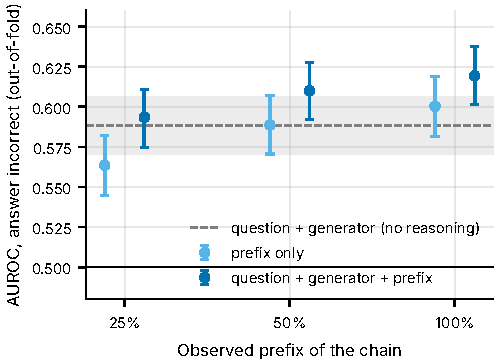
\includegraphics[width=\columnwidth]{fig17_difficulty_control.pdf}
\caption{The prefix adds nothing beyond question and generator until half the chain is observed.}
\label{fig:difficulty}
\end{figure}

\subsection{One first error in four is not fatal}
Fatality of first errors is \fatAll\ [\fatAllLo, \fatAllHi]: \nonFatalPct\% of annotated first errors
are followed by a correct answer (Fig.~\ref{fig:fatality}). Fatality falls with difficulty, from
\fatGsm\ on GSM8K to \fatOmni\ on Omni-MATH, and is flat in the position of the error
(\fatOnsetMin--\fatOnsetMax\ across onset quartiles; \fatLast\ only when the error is in the final
step). Fatal and recovered errors occur at the same relative position (Mann--Whitney $p=\mwRhoP$,
$r=\mwRhoR$).

We read and coded a seeded sample of \codeN\ recovered traces. In \codeFlawed\ the reasoning stays
wrong and the correct answer appears anyway; \codeLowEnt\ have low-entropy or qualitative answers
(yes/no, true/false); in \codeNotLoad\ the error does not bear on the answer; only \codeRepair\
contain a repair; \codeQuest\ flagged step looked correct to the coder. Explicit re-checking
language after the error is barely more frequent in recovered than in fatal traces (\markRec\% vs
\markFat\%, $p=\markP$). Non-fatal errors are thus mostly cases where the written reasoning does not
determine the answer, consistent with~\cite{zhang2025lessons,li2026performative}.

\begin{figure}[t]\centering
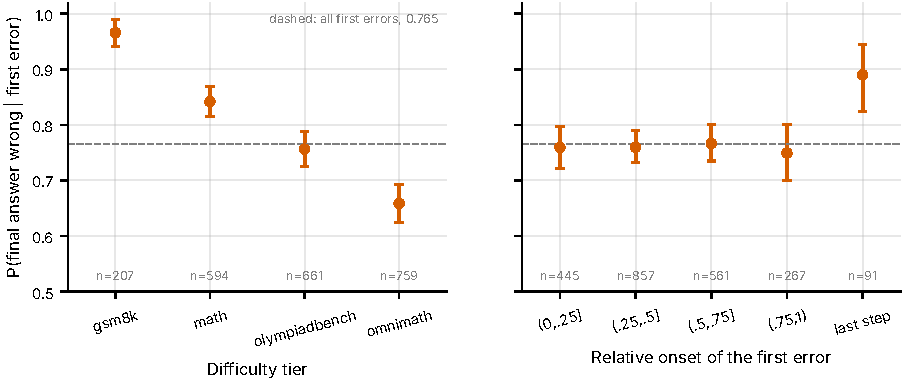
\includegraphics[width=\columnwidth]{fig16_error_fatality.pdf}
\caption{Fatality of first errors by difficulty tier and by where the error occurs.}
\label{fig:fatality}
\end{figure}

\subsection{Detectors track errors, not commitment}
If a failure detector captured commitment, it would score recovered traces like clean ones. It does
the opposite (Table~\ref{tab:threeway}): trained to predict a wrong answer, the full-prefix detector
separates recovered from clean traces (\twOutRC) but ranks fatal traces \emph{below} recovered ones
(\twOutFR\ [\twOutFRLo, \twOutFRHi]); with question and generator included the ranking is at chance
(\twOutQGFR). A detector trained to find errors inverts more strongly (\twErrFR). Among erroneous
traces, the fatality of the first error is predicted by question and generator (AUROC \fatPredQG),
and the error step, the prefix up to it or the next one or two steps change this by at most
\fatPredMaxInc.

\begin{table}[t]\centering\small
\caption{AUROC between outcome groups (positive vs negative).}
\label{tab:threeway}
\begin{tabular}{lccc}\toprule
Detector (trained on) & rec.\ vs clean & fatal vs rec. & fatal vs clean\\\midrule
Prefix 100\% (wrong answer) & \twOutRC & \twOutFR & \twOutFC\\
Q+G+prefix (wrong answer) & \twOutQGRC & \twOutQGFR & \twOutQGFC\\
Prefix 100\% (has error) & \twErrRC & \twErrFR & \twErrFC\\\bottomrule
\end{tabular}
\end{table}

\section{Counterfactual Commitment}\label{sec:counterfactual} (pending)


\section{Discussion}
\textbf{For early warning.} Reported AUROCs for early failure prediction should be accompanied by a
question-only and a generator baseline, the increment over them, and a within-problem concordance;
without them a detector of problem difficulty is indistinguishable from a detector of reasoning
failure. On ProcessBench, text detectors pass this test only after half the chain.

\textbf{For process supervision.} Human first-error labels mark where reasoning first goes wrong,
which is the right target for auditing reasoning. They are not, in general, where the outcome is
decided. Verifiers that are trained or evaluated on first errors and then used to steer search
inherit this gap; the counterfactual value curve measures it directly.

\section{Limitations}
ProcessBench balances answers within each tier, so absolute fatality rates describe the benchmark,
not deployment. The coded sample is small and was coded by one person; we release it for re-coding.
Counterfactual continuations are sampled at temperature 0.7 from models whose original traces were
re-segmented by ProcessBench, so prefixes are near- rather than exactly on-policy. We study
mathematics only, and small open models only.

\section{Conclusion}
Errors are where reasoning first goes wrong; choke points are where it stops being recoverable. On
ProcessBench the two differ often enough, and text-based failure detectors confuse them with problem
difficulty often enough, that both process supervision and early warning should measure the second
directly. The counterfactual value curve does this at the cost of sampling, and its labels are the
natural target for cheaper commitment detectors.

\begin{thebibliography}{99}\small
\bibitem{wei2022cot} J.~Wei, X.~Wang, D.~Schuurmans, M.~Bosma, B.~Ichter, F.~Xia, E.~Chi, Q.~Le, and D.~Zhou, ``Chain-of-thought prompting elicits reasoning in large language models,'' in \emph{NeurIPS}, 2022.
\bibitem{lightman2023} H.~Lightman, V.~Kosaraju, Y.~Burda, H.~Edwards, B.~Baker, T.~Lee, J.~Leike, J.~Schulman, I.~Sutskever, and K.~Cobbe, ``Let's verify step by step,'' arXiv:2305.20050, 2023.
\bibitem{uesato2022} J.~Uesato \emph{et al.}, ``Solving math word problems with process- and outcome-based feedback,'' arXiv:2211.14275, 2022.
\bibitem{wang2024shepherd} P.~Wang \emph{et al.}, ``Math-Shepherd: Verify and reinforce LLMs step-by-step without human annotations,'' in \emph{ACL}, 2024.
\bibitem{processbench} C.~Zheng, Z.~Zhang, B.~Zhang, R.~Lin, K.~Lu, B.~Yu, D.~Liu, J.~Zhou, and J.~Lin, ``ProcessBench: Identifying process errors in mathematical reasoning,'' in \emph{ACL}, 2025.
\bibitem{zhang2025lessons} Z.~Zhang \emph{et al.}, ``The lessons of developing process reward models in mathematical reasoning,'' arXiv:2501.07301, 2025.
\bibitem{tyen2024} G.~Tyen, H.~Mansoor, V.~C\u{a}rbune, P.~Chen, and T.~Mak, ``LLMs cannot find reasoning errors, but can correct them given the error location,'' in \emph{Findings of ACL}, 2024.
\bibitem{huang2024} J.~Huang, X.~Chen, S.~Mishra, H.~S.~Zheng, A.~W.~Yu, X.~Song, and D.~Zhou, ``Large language models cannot self-correct reasoning yet,'' in \emph{ICLR}, 2024.
\bibitem{afzal2025} A.~Afzal, F.~Matthes, G.~Chechik, and Y.~Ziser, ``Knowing before saying: LLM representations encode information about chain-of-thought success before completion,'' arXiv:2505.24362, 2025.
\bibitem{lugoloobi2026} W.~Lugoloobi, T.~Foster, W.~Bankes, and C.~Russell, ``LLMs encode their failures: Predicting success from pre-generation activations,'' arXiv:2602.09924, 2026.
\bibitem{bulut2026} Y.~U.~Bulut, ``It's the problem, not the path: Budget and difficulty confounds in LLM reasoning trajectories,'' arXiv:2609.03436, 2026.
\bibitem{bogdan2025} P.~C.~Bogdan, U.~Macar, N.~Nanda, and A.~Conmy, ``Thought anchors: Which LLM reasoning steps matter?'' arXiv:2506.19143, 2025.
\bibitem{lin2025critical} Z.~Lin \emph{et al.}, ``Critical tokens matter: Token-level contrastive estimation enhances LLM's reasoning capability,'' in \emph{ICML}, 2025.
\bibitem{bigelow2025} E.~Bigelow, A.~Holtzman, H.~Tanaka, and T.~Ullman, ``Forking paths in neural text generation,'' in \emph{ICLR}, 2025.
\bibitem{liao2025lost} B.~Liao \emph{et al.}, ``Lost at the beginning of reasoning,'' arXiv:2506.22058, 2025.
\bibitem{merrill2026} S.~Merrill and S.~Srivastava, ``The point of no return: Counterfactual localization of deceptive commitment in language-model reasoning,'' arXiv:2605.17113, 2026.
\bibitem{jiang2026ocr} D.~Jiang, Z.~Zhang, K.~Yuan, and S.~Ma, ``Not every divergence should be suppressed: Counterfactual recoverability in on-policy distillation,'' arXiv:2608.04408, 2026.
\bibitem{li2026performative} W.~Li, F.~Yang, A.~Hazarika, S.~A.~Mehta, and K.~Onoue, ``When reasoning traces become performative: Step-level evidence that chain-of-thought is an imperfect oversight channel,'' arXiv:2605.11746, 2026.
\bibitem{boppana2026} S.~Boppana \emph{et al.}, ``Reasoning theater: Disentangling model beliefs from chain-of-thought,'' arXiv:2603.05488, 2026.
\bibitem{cheung2026crop} M.~Y.~Cheung, A.~Veeraraghavan, H.~Chen, and G.~Balakrishnan, ``Conformal certification of reasoning trace prefixes,'' arXiv:2605.30085, 2026.
\bibitem{orgad2024} H.~Orgad \emph{et al.}, ``LLMs know more than they show: On the intrinsic representation of LLM hallucinations,'' arXiv:2410.02707, 2024.
\bibitem{kadavath2022} S.~Kadavath \emph{et al.}, ``Language models (mostly) know what they know,'' arXiv:2207.05221, 2022.
\bibitem{wang2023sc} X.~Wang, J.~Wei, D.~Schuurmans, Q.~Le, E.~Chi, S.~Narang, A.~Chowdhery, and D.~Zhou, ``Self-consistency improves chain of thought reasoning in language models,'' in \emph{ICLR}, 2023.
\bibitem{qwen25} A.~Yang \emph{et al.}, ``Qwen2.5 technical report,'' arXiv:2412.15115, 2024.
\bibitem{qwen25math} A.~Yang \emph{et al.}, ``Qwen2.5-Math technical report: Toward mathematical expert model via self-improvement,'' arXiv:2409.12122, 2024.
\bibitem{vllm} W.~Kwon \emph{et al.}, ``Efficient memory management for large language model serving with PagedAttention,'' in \emph{SOSP}, 2023.
\bibitem{field2007} C.~A.~Field and A.~H.~Welsh, ``Bootstrapping clustered data,'' \emph{J. R. Stat. Soc. B}, vol.~69, no.~3, pp.~369--390, 2007.
\bibitem{tfidf} F.~Pedregosa \emph{et al.}, ``Scikit-learn: Machine learning in Python,'' \emph{JMLR}, vol.~12, pp.~2825--2830, 2011.
\end{thebibliography}

\end{document}
